
%  XXX XXX XXX  THIS IS A NEW FILE XXX XXX XXX

%
% /home/visesh/Papers/ICCV15/FiducialMallikarjun/deva_modification.tex
%
% Developed by @AUTHOR@ <@EMAIL@>
% Copyright (c) 2015 @COMPANY@
% Licensed under terms of GNU General Public License.
% All rights reserved.
%
% Changelog:
% 22/04/2015 - created
%

% $Platon$

\begin{figure}
  \centering
  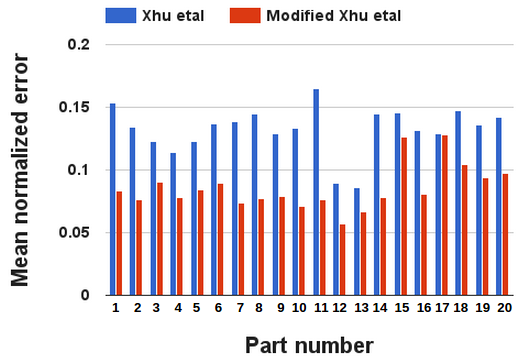
\includegraphics[width=4.3in,height=2.8in]{fid/figures/deva_modification_parts_mean_error2.png}
  \caption{Comparison between Zhu \etal~\cite{xhuCVPR12_wild} (blue bars), and its modification
  using our exemplar approach (red bars). For each part, the y-axis plots the mean pixel error
  normalized by interocular distance over the entire COFW dataset.}
\end{figure}

\label{sec:modification_xhu}
We modify Zhu \etal~\cite{xhuCVPR12_wild} approach by replacing feature pyramid constructed using the HoG filters for each part which represents the likelihood of part location, 
by response based on the feature distance at each pixel in euclidean space with respect to corresponding feature of the part in the exemplars. 
Here we restrict the likelihood area for each part in the response within the boundary which
encloses the prediction of corresponding part in candidate
methods that we use. The likelihood score is inversely proportional to the distance of the feature at each pixel with respect to the corresponding part 
in the exemplar. Within that boundary, we compute the feature based on SIFT and HoG and compute the distance with respect to the feature computed 
at corresponding part in 20 exemplars. We choose the smallest distance among them to score the likelihood for that pixel. 
With this modification we see significant reduction in the failure rate and mean error of Zhu
\etal~\cite{xhuCVPR12_wild} in COFW dataset which has lot of occluded faces.
